\documentclass[tikz,border=10pt]{standalone}
\usepackage{tikz}
\usetikzlibrary{shapes, decorations.pathmorphing, decorations.pathreplacing, decorations.markings, patterns, calc}

\begin{document}
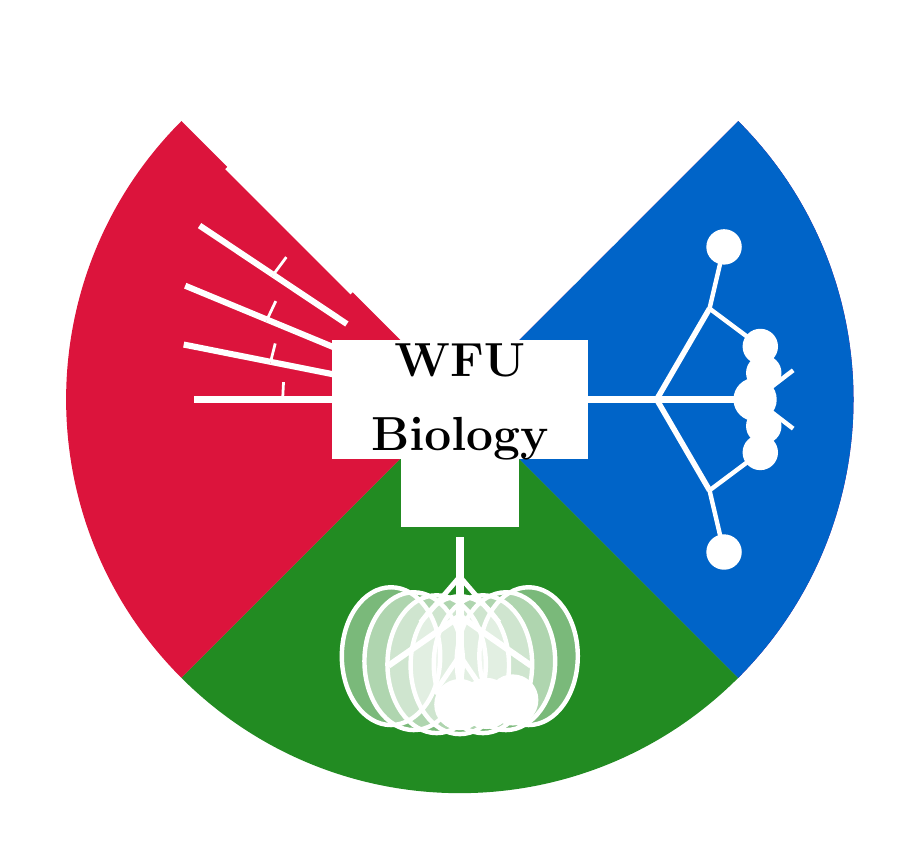
\begin{tikzpicture}[scale=2.5]

% Define colors - matching the reference image
\definecolor{red}{RGB}{220,20,60}
\definecolor{purple}{RGB}{128,0,128}
\definecolor{green}{RGB}{34,139,34}
\definecolor{blue}{RGB}{0,100,200}

% Draw the four corner wedges arranged around center
% Each wedge is a quarter circle segment

% Top-left wedge: Red with DNA helix (135° to 225°)
\fill[red] (0,0) -- (135:2) arc (135:225:2) -- cycle;

% DNA double helix in top-left wedge
% Create a more accurate DNA helix representation
\foreach \i in {0,1,2,3,4,5,6,7} {
    \pgfmathsetmacro{\angle}{180-\i*11.25}
    \pgfmathsetmacro{\angleconn}{180-(\i+0.5)*11.25}
    \pgfmathsetmacro{\radius}{0.9+\i*0.08}
    % Left strand
    \draw[white, line width=2.2pt] 
        (\angle:\radius) .. controls (\angle:\radius+0.15) and (\angle:\radius+0.3) .. (\angle:\radius+0.45);
    % Right strand  
    \draw[white, line width=2.2pt] 
        (\angle:\radius) .. controls (\angle:\radius-0.15) and (\angle:\radius-0.3) .. (\angle:\radius-0.45);
    % Connecting rungs between strands
    \draw[white, line width=1pt] (\angle:\radius) -- (\angleconn:\radius);
}

% Top-right wedge: Purple with brain (45° to -45°)
\fill[purple] (0,0) -- (45:2) arc (45:-45:2) -- cycle;

% Brain line drawing in top-right wedge
% Create a more anatomically accurate brain shape
\draw[white, line width=2.8pt] 
    (0:1.0) 
    .. controls (20:0.95) and (35:0.9) .. (45:0.85)
    .. controls (35:0.75) and (20:0.65) .. (0:0.6)
    .. controls (-20:0.65) and (-35:0.75) .. (-45:0.85)
    .. controls (-35:0.9) and (-20:0.95) .. (0:1.0)
    .. controls (20:1.1) and (35:1.15) .. (45:1.12)
    .. controls (35:1.08) and (20:1.03) .. (0:0.98)
    .. controls (-20:1.03) and (-35:1.08) .. (-45:1.12)
    .. controls (-35:1.15) and (-20:1.1) .. cycle;
% Brain texture - gyri and sulci (folds)
\foreach \i in {-40,-25,-10,10,25,40} {
    \draw[white, line width=1.3pt] 
        (\i:0.7) .. controls (\i:0.85) and (\i:0.95) .. (\i:1.02);
}

% Bottom-left wedge: Green with vine and leaves (225° to 315°)
\fill[green] (0,0) -- (225:2) arc (225:315:2) -- cycle;

% Vine with leaves in bottom-left wedge
% Main vine stem
\draw[white, line width=2.8pt] (270:0.7) -- (270:1.6);
% Primary branches
\draw[white, line width=2.2pt] (270:1.1) -- (255:1.4);
\draw[white, line width=2.2pt] (270:1.1) -- (285:1.4);
% Secondary branches
\draw[white, line width=1.8pt] (270:0.9) -- (260:1.15);
\draw[white, line width=1.8pt] (270:0.9) -- (280:1.15);
\draw[white, line width=1.8pt] (270:1.3) -- (265:1.5);
\draw[white, line width=1.8pt] (270:1.3) -- (275:1.5);
% Leaves - more natural leaf shapes
\foreach \angle in {255,260,265,270,275,280,285} {
    \draw[white, fill=white, fill opacity=0.4, line width=1.6pt] 
        (\angle:1.35) ellipse (0.25 and 0.35);
}
% Small berries/buds
\foreach \angle in {270,275,280} {
    \fill[white] (\angle:1.55) circle (0.13);
}

% Bottom-right wedge: Blue with phylogenetic tree (315° to 45°)
\fill[blue] (0,0) -- (315:2) arc (315:405:2) -- cycle;

% Phylogenetic tree in bottom-right wedge
% Main trunk
\draw[white, line width=2.2pt] (0:0.65) -- (0:1.5);
% Left major branch
\draw[white, line width=2pt] (0:1.0) -- (-20:1.35);
% Right major branch  
\draw[white, line width=2pt] (0:1.0) -- (20:1.35);
% Left sub-branches
\draw[white, line width=1.6pt] (-20:1.35) -- (-30:1.55);
\draw[white, line width=1.6pt] (-20:1.35) -- (-10:1.55);
% Right sub-branches
\draw[white, line width=1.6pt] (20:1.35) -- (10:1.55);
\draw[white, line width=1.6pt] (20:1.35) -- (30:1.55);
% Top branches
\draw[white, line width=1.6pt] (0:1.5) -- (-5:1.7);
\draw[white, line width=1.6pt] (0:1.5) -- (5:1.7);
% Terminal nodes (species/tips)
\foreach \angle in {-30,-10,-5,5,10,30} {
    \fill[white] (\angle:1.55) circle (0.09);
}
\fill[white] (0:1.5) circle (0.11);

% Central white cross area - creates gaps between wedges
% Vertical bar
\fill[white] (-0.3,-0.65) rectangle (0.3,0.65);
% Horizontal bar
\fill[white] (-0.65,-0.3) rectangle (0.65,0.3);

% Text in center: "WFU Biology"
\node[text=black, font=\bfseries\LARGE, align=center] at (0,0.2) {WFU};
\node[text=black, font=\bfseries\LARGE, align=center] at (0,-0.2) {Biology};

\end{tikzpicture}
\end{document}
